\section{Automatic generation of JIT compilers}

Traditional JIT compilers are hard to write, time consuming and hard to
evolve.  On the other hand, interpreters are easy both to write and maintain,
but they are usually slow.  By automatically generating a JIT compiler out of
an interpreter, we take the best of both worlds.

\commentout{
\begin{figure}[h]
\begin{center}
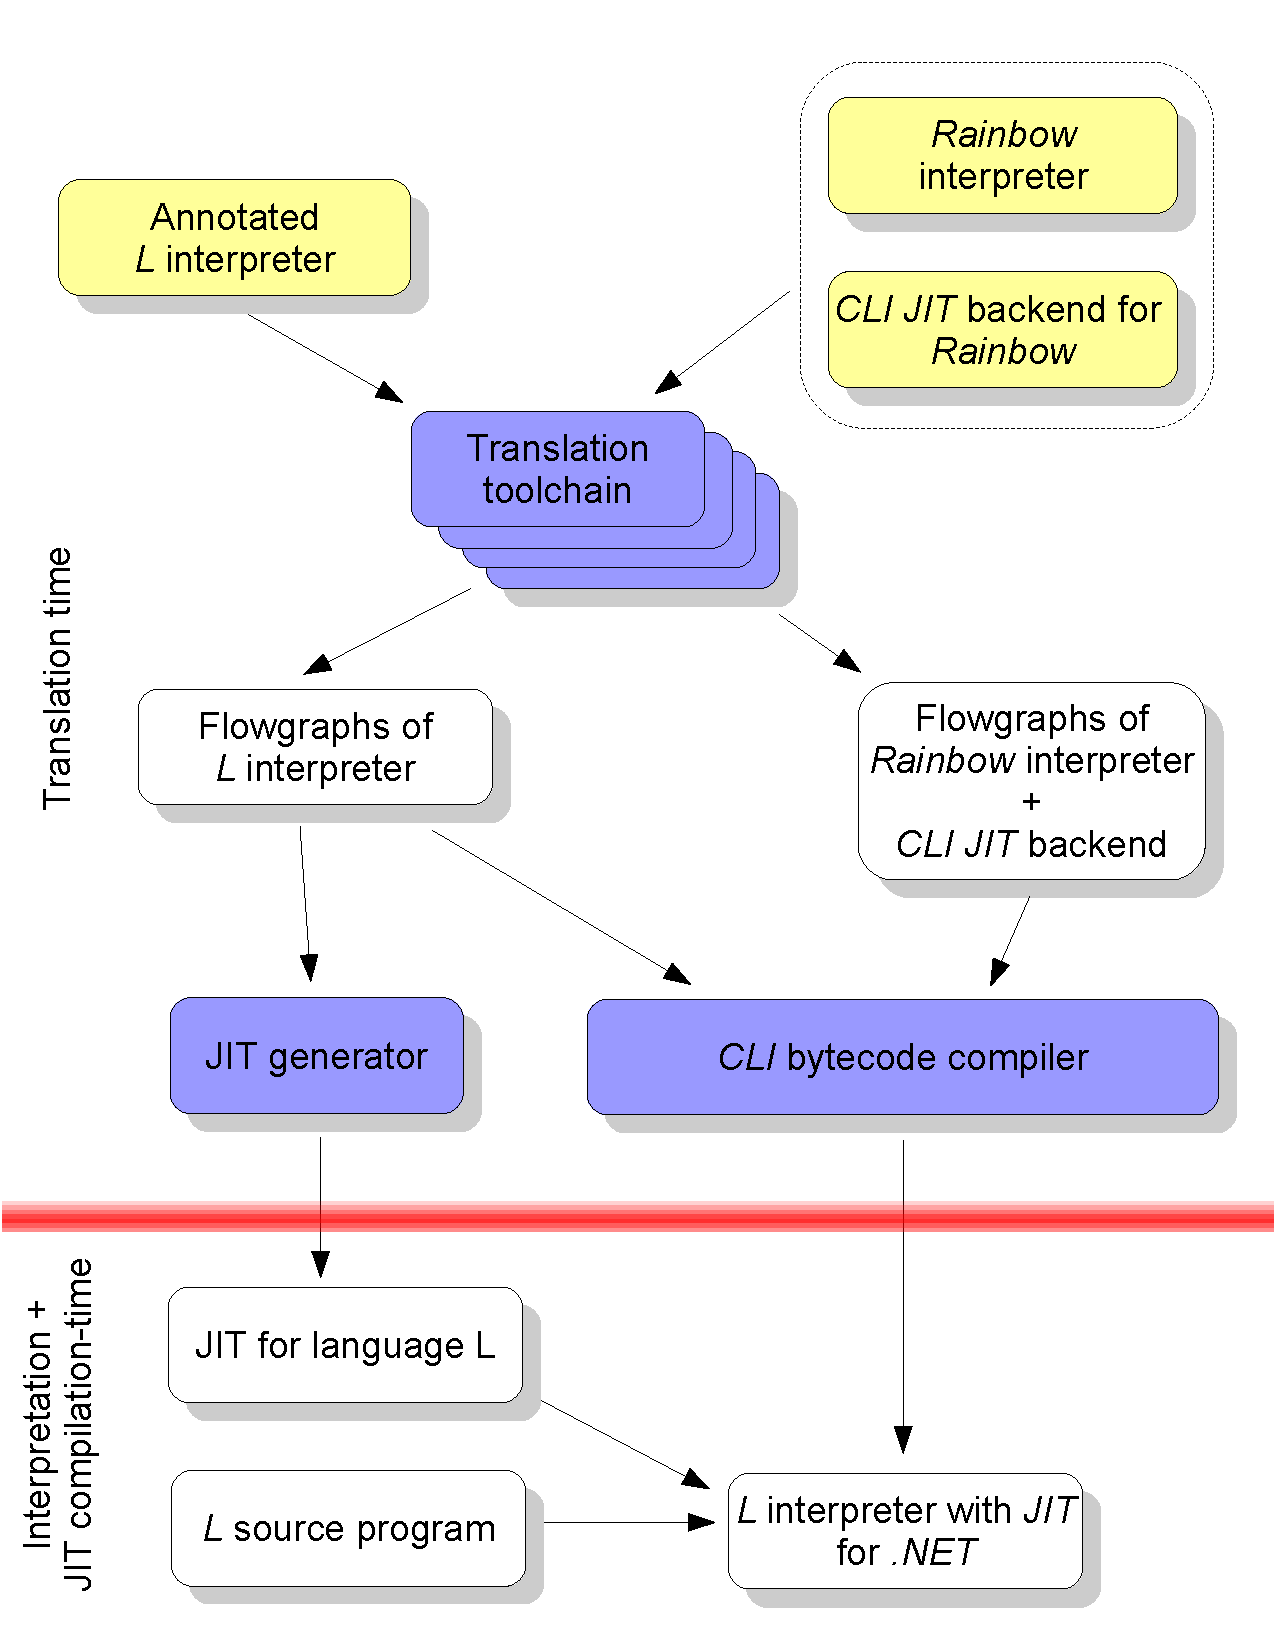
\includegraphics[width=.6\textwidth]{diagram1}
\caption{PyPy infrastructure for generating an interpreter of a
  language $L$ with JIT compilation for the .NET platform}
\end{center}
\end{figure}
}

The JIT generation framework uses partial evaluation techniques to generate a
dynamic compiler from an interpreter; the idea is inspired by Psyco \cite{DBLP:conf/pepm/Rigo04}, which
uses the same techniques but it's manually written instead of being
automatically generated.

\subsection{Partial evaluation}

Yoshihiko Futamura published a paper \cite{Futamura99} that proposed a
technique to automatically transform an interpreter of a programming language
into a compiler for the same language. This would solve the problem of having to
write a compiler instead of a much simpler interpreter. He proposed to use
partial evaluation to achieve this goal. He defined partial evaluation along the following lines:

Given a program $P$ with $m + n$ input variables $s_1, ..., s_m$ and $d_1, ...,
d_n$, the partial evaluation of $P$ with respect to concrete values $s'_1, ...,
s'_m$ for the first $m$ variables is a program $P'$. The program $P'$ takes only
the input variables $d_1, ..., d_n$ but behaves exactly like $P$ with the
concrete values (but is hopefully more efficient). This transformation is done
by a program $S$, the partial evaluator, which takes $P$ and $s_1, ..., s_m$ as
input:

    $$S(P, (s'_1, ..., s'_m)) = P'$$

The variables $s_1, ..., s_m$ are called the \emph{static} variables, the
variables $d_1, ..., d_n$ are called the \emph{dynamic} variables; $P'$ is the
\emph{residual code}. Partial evaluation creates a version of $P$ that works
only for a fixed set of inputs for the first $m$ arguments. This effect is
called \emph{specialization}.

When $P$ is an interpreter for a programming language, then the $s_1, ..., s_m$
are chosen such that they represent the program that the interpreter is
interpreting and the $d_1, ..., d_n$ represent the input of this program. Then
$P'$ can be regarded as a compiled version of the program that the chosen $s'_1,
..., s'_m$ represent, since it is a version of the interpreter that can only
interpret this program. Now once the partial evaluator $S$ is implemented, it is
actually enough to implement an interpreter for a new language and use $S$
together with this interpreter to compile programs in that new language.

A valid implementation for $S$ would be to just put the concrete values into $P$
to get $P'$, which would not actually produce any performance benefits compared with
directly using $P$. A good implementation for $S$ should instead make use of the
information it has and evaluate all the parts of the program that actually
depend only on the $s_1, ..., s_m$ and to remove parts of $P$ that cannot be
reached given the concrete values.

\begin{figure}[h]
\begin{center}
\input{tlc-simplified.py}
\caption{The main loop of the TLC interpreter, written in RPython}
\label{fig:tlc-main}
\end{center}
\end{figure}

Let us look at an example. Figure \ref{fig:tlc-main} shows parts of the
main-loop of the TLC interpreter (in slightly simplified form). The static
arguments of this functions would typically be the \lstinline{code} argument
(containing the bytecode as a string), the \lstinline{pc} argument (containing
the initial program counter) and the \lstinline{pool} argument (containing the
constant pool). The \lstinline{args} argument is dynamic since it contains the
user-input of the interpreted function. Since the \lstinline{while} loop and the
contained conditions depend only on static arguments it will typically be
unrolled by a partial evaluator.

When the function is partially evaluated with respect to the TLC example
function shown in Figure \ref{fig:tlc-abs} (which computes the absolute value of a number),
the residual code would look like in Figure \ref{fig:tlc-folded}. This version
is already a great improvement over pure interpretation, all the bytecode
dispatch overhead has been removed. However, the function as shown is still
rather inefficient, due to lots of superfluous stack handling and also due to
some indirect calls for implementing comparison (\lstinline{lt}) and
subtraction (\lstinline{sub}).

\begin{figure}[h]
\begin{center}
\input{tlc-folded.py}
\caption{The residual code of the TLC main loop with respect to the
\lstinline{abs} function }
\label{fig:tlc-folded}
\end{center}
\end{figure}

This shows a common shortcoming of partial evaluation when applied to a dynamic
language: The partial evaluator (just like an ahead-of-time compiler) cannot
make assumptions about the types of objects, which leads to poor results.
Effective dynamic compilation requires feedback of runtime information into
compile-time. This is no different for partial evaluation, and subsequent sections shows how we managed to solve this problem.


\subsection{Binding Time Analysis in PyPy}

At translation time, PyPy performs binding-time analysis of the source RPython
program, to determine which variables are static and which dynamic.  The
binding-time terminology that we are using in PyPy is based on the colors that
we use when displaying the control flow graphs:

\begin{itemize}
\item \emph{Green} variables contain values that are known at compile-time.
They correspond to static arguments.
\item \emph{Red} variables contain values that are usually not known
compile-time. They correspond to dynamic arguments.
\end{itemize}

The binding-time analyzer of our translation tool-chain is using a simple
abstract-interpretation based analysis. It is based on the
same type inference engine that is used on the source RPython program.
This is called the \emph{hint-annotator}; it
operates over input flowgraphs
and propagates annotations that do not track types but
value dependencies and manually-provided binding time hints.

The normal process of the hint-annotator is to propagate the binding
time (i.e. color) of the variables using the following kind of rules:

\begin{itemize}
\item For a foldable operation (i.e. one without side effect and which depends
only on its argument values), if all arguments are green, then the result can
be green too.

\item Non-foldable operations always produce a red result.

\item At join points, where multiple possible values (depending on control
flow) are meeting into a fresh variable, if any incoming value comes from a red
variable, the result is red.  Otherwise, the color of the result might be
green.  We do not make it eagerly green, because of the control flow
dependency: the residual function is basically a constant-folded copy of the
source function, so it might retain some of the same control flow.  The value
that needs to be stored in the fresh join variable thus depends on which
branches are taken in the residual graph.
\end{itemize}

\subsection{Hints}
\label{sec:hints}

Our goal in designing our approach to binding-time analysis was to
minimize the number of explicit hints that the user must provide in
the source of the RPython program.  This minimalism was not pushed to
extremes, though, to keep the hint-annotator reasonably simple.  

The driving idea was that hints should be need-oriented.  Indeed, in a
program like an interpreter, there are a small number of places where it
would be clearly beneficial for a given value to be known at
compile-time, i.e. green: this is where we require the hints to be
added.

The hint-annotator assumes that all variables are red by default, and
then propagates annotations that record dependency information.
When encountering the user-provided hints, the dependency information
is used to make some variables green.  All
hints are in the form of an operation \texttt{hint(v1, someflag=True)}
which semantically just returns its first argument unmodified.

The crucial need-oriented hint is \texttt{v2 = hint(v1, concrete=True)}
which should be used in places where the programmer considers the
knowledge of the value to be essential.  This hint is interpreted by
the hint-annotator as a request for both \texttt{v1} and \texttt{v2} to be green.  It
has a \emph{global} effect on the binding times: it means that not only
\texttt{v1} but all the values that \texttt{v1} depends on – recursively –
are forced to be green.  The hint-annotator gives an error if the
dependencies of \texttt{v1} include a value that cannot be green, like
a value read out of a field of a non-immutable instance.

Such a need-oriented backward propagation has advantages over the
commonly used forward propagation, in which a variable is compile-time
if and only if all the variables it depends on are also compile-time.  A
known issue with forward propagation is that it may mark as compile-time
either more variables than expected (which leads to over-specialization
of the residual code), or less variables than expected (preventing
specialization to occur where it would be the most useful).  Our
need-oriented approach reduces the problem of over-specialization, and
it prevents under-specialization: an unsatisfiable \texttt{hint(v1,
concrete=True)} is reported as an error.

There are cases in which having a green variable is essential for generating
good code, but it is not possible to use the \texttt{concrete} hint due to an
unsatisfiable dependency: Section~\ref{sec:promotion} introduces
\emph{promotion}, the novel technique that makes possible to solve this
problem.
